\documentclass[aspectratio=169]{beamer} %% for 16:9 use this line
%%\documentclass{beamer} %% For 4:3 ratio use this line
\usepackage[utf8]{inputenc}
\usepackage[T1]{fontenc}
\usepackage{lipsum} 
\usepackage{bm}
\usepackage{graphicx}
\usepackage{animate}
\usepackage{amsmath}
\usepackage{subcaption}
\usepackage{tikz}
\usepackage{soul}
\usepackage[most]{tcolorbox}
\usepackage{amssymb}% http://ctan.org/pkg/amssymb
\usepackage{pifont}% http://ctan.org/pkg/pifont
\newcommand{\cmark}{\ding{51}}%
\newcommand{\xmark}{\ding{55}}%
\captionsetup[figure]{font=footnotesize}
% import citation package
\usepackage[backend=biber, style=authoryear]{biblatex}
\addbibresource{../../conference/biblio.bib}
\AtBeginBibliography{\small}
\DeclareMathOperator*{\argmin}{\arg\!\min}
% footnote without number
\newcommand\blfootnote[1]{
\begingroup
\renewcommand\thefootnote{}\footnote{#1}
\addtocounter{footnote}{-1}
\endgroup
}

\usetheme{CEA2023}
\setlength{\columnsep}{0.05cm}
\title[Café Thésard]
{Marius Duvillard - Construction du jumeau numérique du procédé de mélange/broyage des combustibles par assimilation de données} %optional
\subtitle{Café Thésard 28/06/2024}
\date[28-06-2024] %optional
{28 juin 2024}
\author[M. Duvillard] %optionam
{Marius Duvillard \inst{1} \inst{2} \texttt{(\small marius.duvillard\myat cea.fr)} \\
Olivier Le Maître \inst{2} \inst{3} \texttt{(\small olivier.le-maitre\myat polytechnique.edu)} \\
Jérémie Bruyelle \inst{1} \texttt{(\small jeremie.bruyelle\myat cea.fr)}\\
}

\institute[short-inst]{
 \inst{1} CEA DES/IRESNE/DEC/SESC Cadarache 
 \inst{2} Centre de Mathématiques Appliquées, Ecole Polytechnique 
 \inst{3} CNRS, Inria
}

% uncomment the following lines if you do not want dedicated outlines before
% each section
\AtBeginSection{}

% use your thanks-message in the last frame
\setvalue{\ThxMessage}{Thanks! Any questions?}
% Change the logo 
\titlegraphic{logos/LOGO_CEA_ORIGINAL.png}

% introduce another logo for a second author or affiliation
% secondlogo applies to the first page only
\setvalue{\secondlogo}{logos/Polytechnique_logo.pdf}

\begin{document}

%11.3 présenter la correction
\begin{frame}{Application - assimilation}
    \begin{figure}[t]
        \centering
        \begin{subfigure}{0.3\textwidth}
            \centering
            \alt<2>{%
                \animategraphics[loop, autoplay, height=0.3\textheight]{100}{../../conference/images/dipole_estimate/reference/reference-}{0}{4}%0}
            }
            {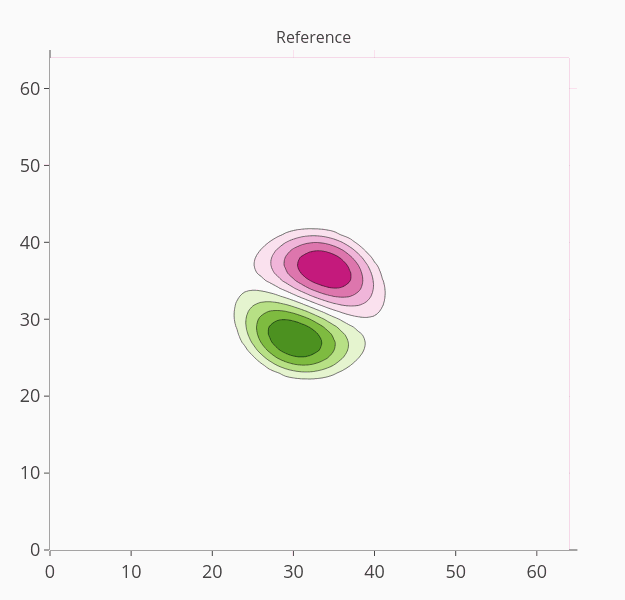
\includegraphics[height=0.3\textheight]{../../conference/images/dipole_estimate/reference/reference-0.png}}
            \caption*{\tiny référence}
        \end{subfigure}
        \begin{subfigure}{0.3\textwidth}
            \centering
            \alt<2>{%
                \animategraphics[loop, autoplay, height=0.3\textheight]{100}{../../conference/images/dipole_estimate/obs_no_noise/obs_no_noise-}{0}{1}%9}
            }
            {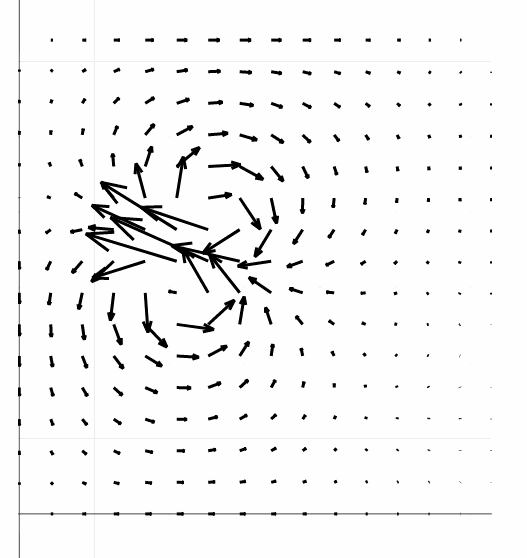
\includegraphics[height=0.3\textheight]{../../conference/images/dipole_estimate/obs_no_noise/obs_no_noise-0.png}}
            \caption*{\tiny champ de vitesse}
        \end{subfigure}
        \begin{subfigure}{0.3\textwidth}
            \centering
            \alt<2>{%
                \animategraphics[loop, autoplay, height=0.3\textheight]{100}{../../conference/images/dipole_estimate/obs_noise/obs_noise-}{0}{1}%9}
            }
            {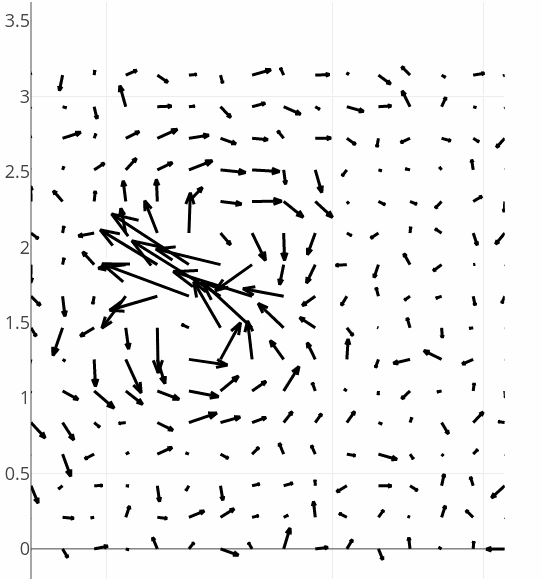
\includegraphics[height=0.3\textheight]{../../conference/images/dipole_estimate/obs_noise/obs_noise-0.png}}
            \caption*{\tiny champ de vitesse bruité}
        \end{subfigure}
    \end{figure}
    \begin{figure}[t]
        \begin{subfigure}{0.3\textwidth}
            \centering
            \alt<2>{%
                \animategraphics[loop, autoplay, height=0.3\textheight]{100}{../../conference/images/dipole_estimate/estimate/estimate-}{0}{4}%0}
            }
            {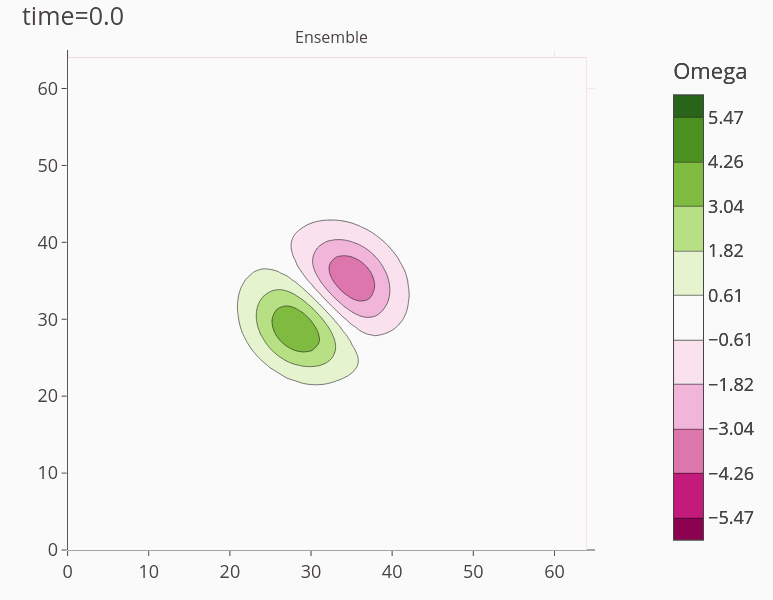
\includegraphics[height=0.3\textheight]{../../conference/images/dipole_estimate/estimate/estimate-0.png}}
            \caption*{\tiny estimateur}
        \end{subfigure}
        \begin{subfigure}{0.3\textwidth}
            \centering
            \alt<2>{%
                \animategraphics[loop, autoplay, height=0.3\textheight]{100}{../../conference/images/dipole_estimate/ensemble_sample/ensemble_sample-}{0}{4}%0}
            }
            {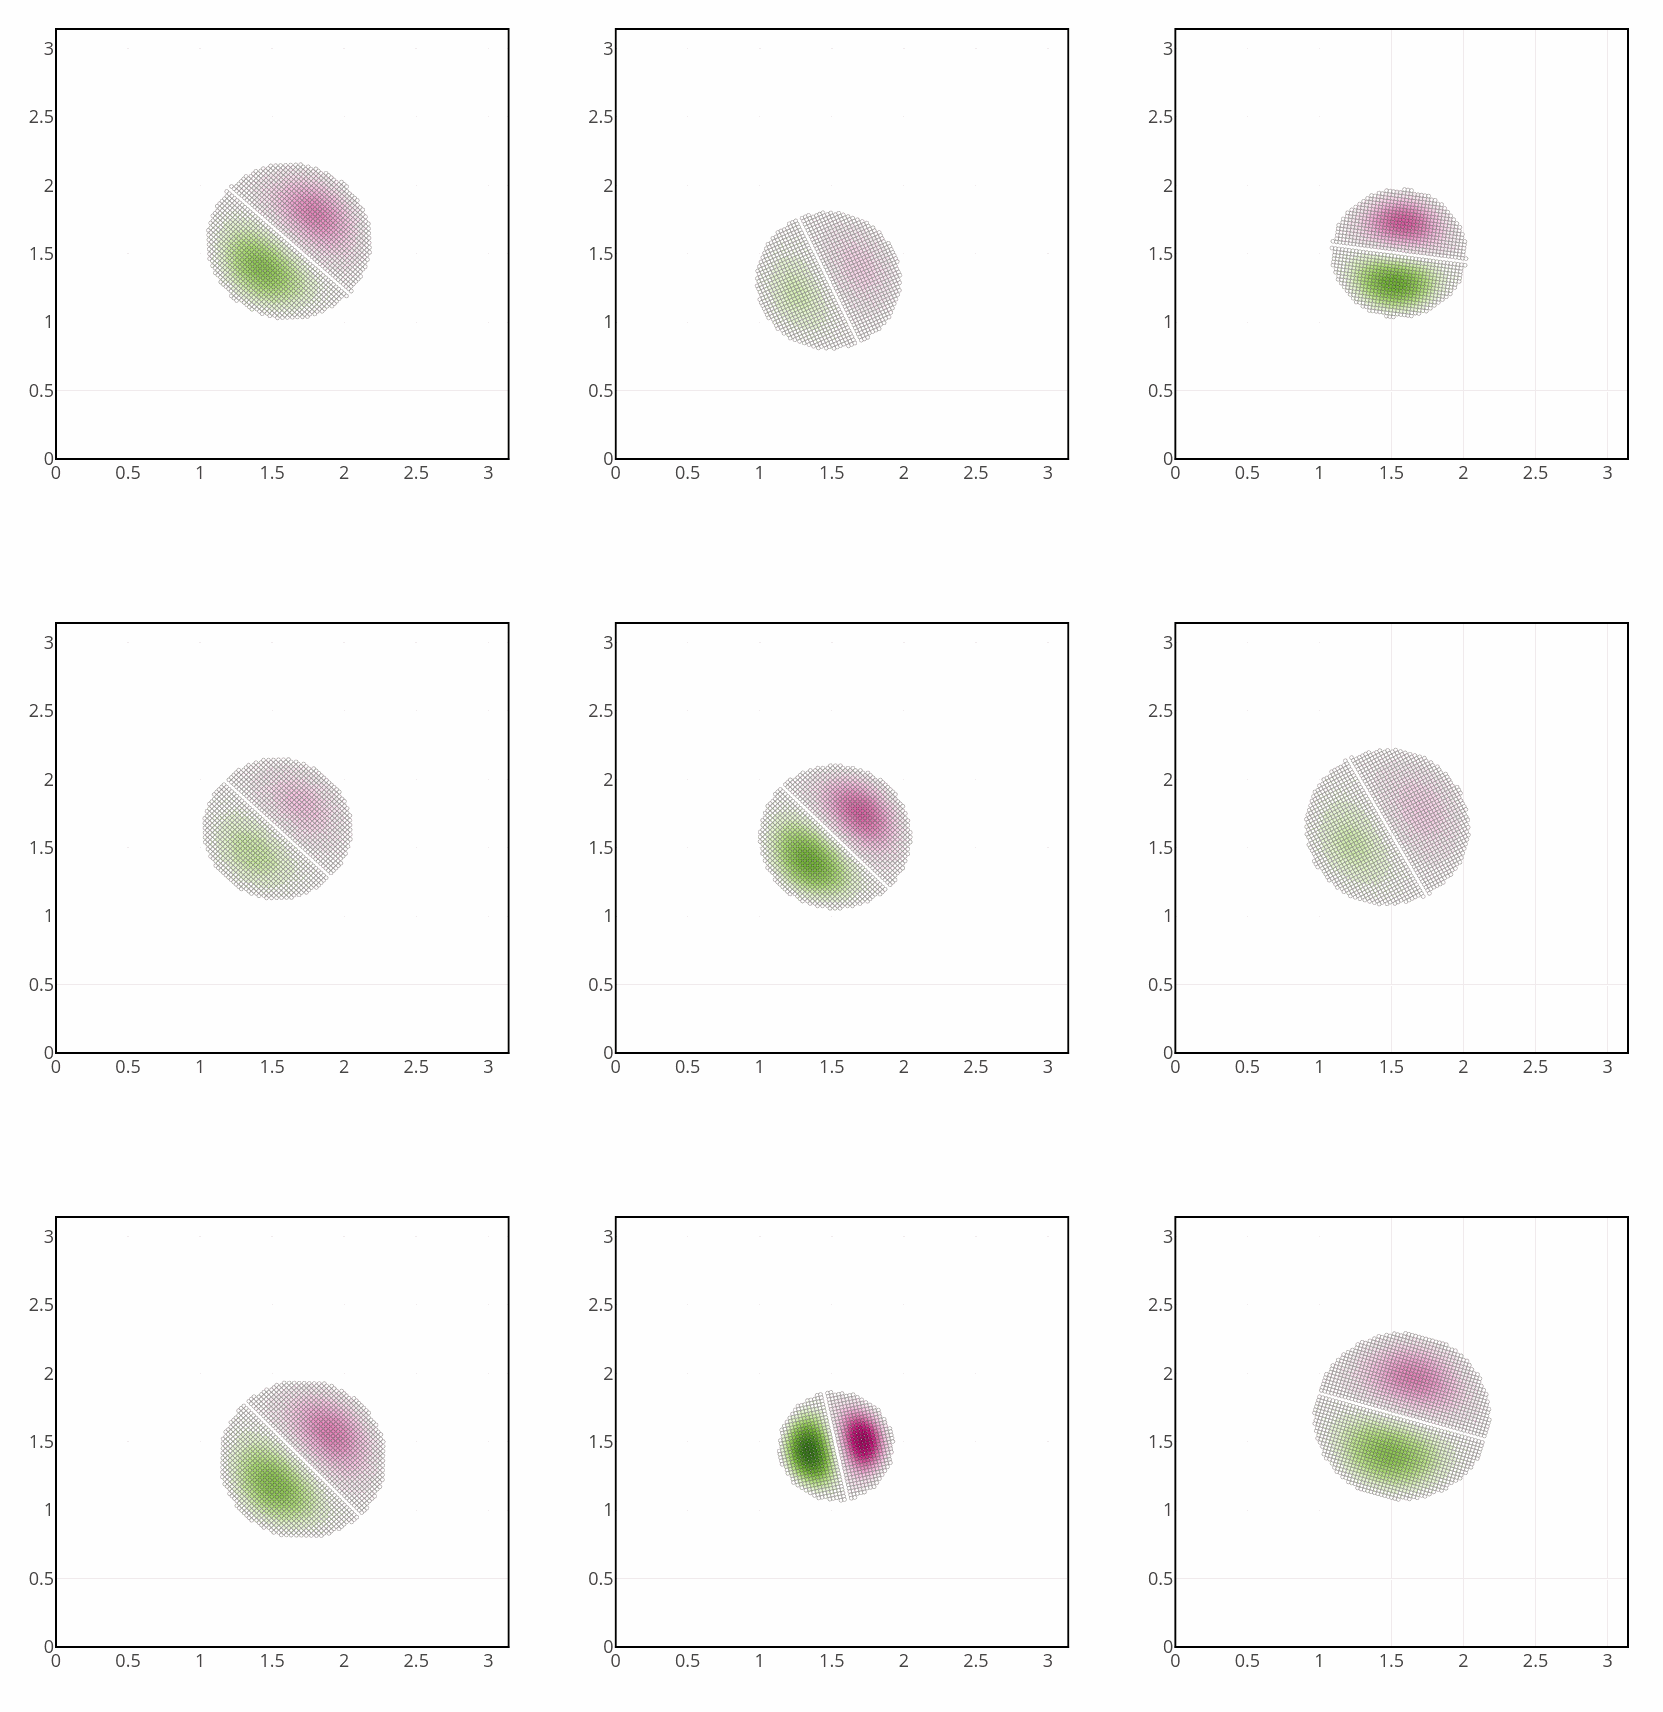
\includegraphics[height=0.3\textheight]{../../conference/images/dipole_estimate/ensemble_sample/ensemble_sample-0.png}}
            \caption*{\tiny échantillons}
        \end{subfigure}
        \hfill
    \end{figure}

    \begin{tikzpicture}[overlay, remember picture]
        \coordinate (Mid1) at (-2,4.5);
        \coordinate (Mid2) at (16, 4.5);
        \coordinate (Im1b) at (4.2,6.75);
        \coordinate (Im2a) at (5.6,6.75);
        \coordinate (Im2b) at (8.2,6.75);
        \coordinate (Im3a) at (10,6.75);
        \coordinate (Im3b) at (11.5,4.5);
        \coordinate (Im3ba) at (11.5,2.25);
        \coordinate (Im4a) at (10.8,2.25);
        \coordinate (Im4b) at (7.9,2.25);
        \coordinate (Im5a) at (6.5,2.25);


        \coordinate (B) at (16,9);
        \draw[->, thick, ceared] (Im1b) -- (Im2a);
        \draw[->, thick, ceared] (Im2b) -- (Im3a);
        \draw[-, thick, ceared] (Im3b) -- (Im3ba);
        \draw[->, thick, ceared] (Im3ba) -- (Im4a);
        \draw[->, thick, ceared] (Im4b) -- (Im5a);

        \draw[->, dashed, ceared] (Mid1) -- (Mid2);

    \end{tikzpicture}
\end{frame}

%11.4 présenter les courbes 
\begin{frame}{Résultats}

    \begin{figure}
        \begin{subfigure}{0.49\textwidth}
            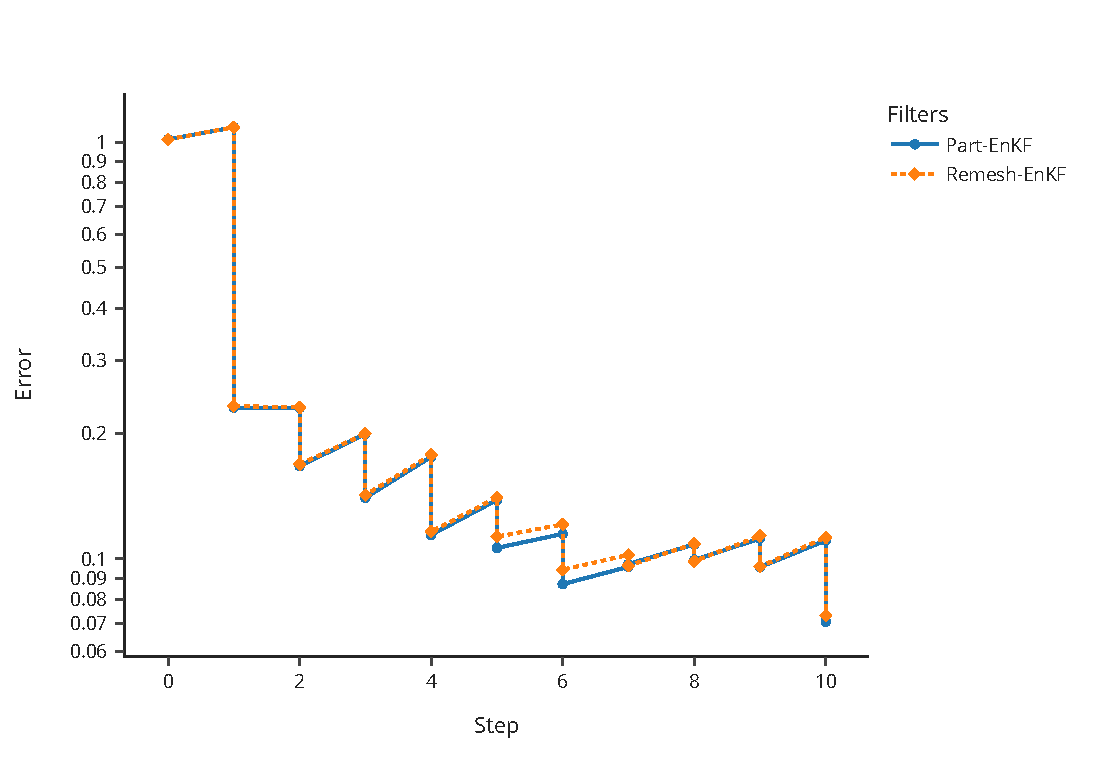
\includegraphics[width=\textwidth]{../../conference/images/dipole_results/error_in_time.pdf}
            \caption*{évolution de l'erreur du champ de tourbillon}
        \end{subfigure}
        \begin{subfigure}{0.49\textwidth}
            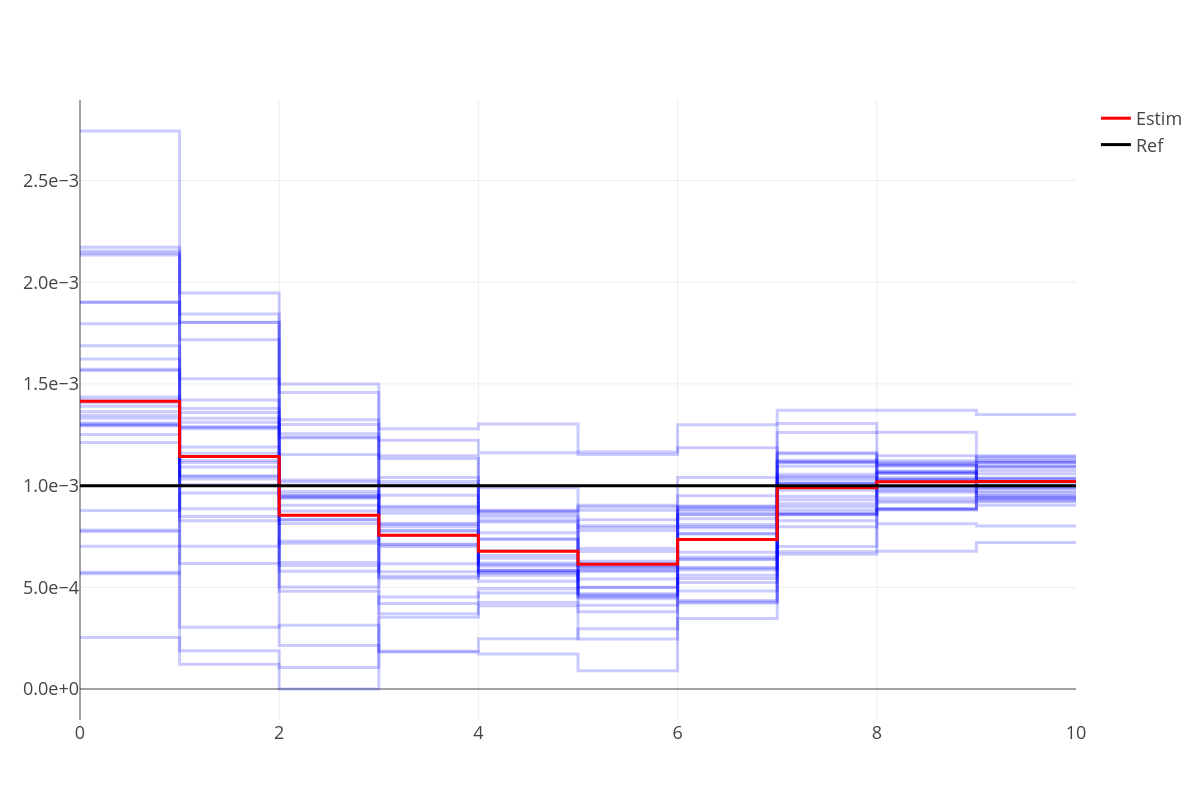
\includegraphics[width=\textwidth]{../../conference/images/dipole_results/visc_rmf.png}
            \caption*{calibration de la viscosité $\nu$}
        \end{subfigure}
    \end{figure}
\end{frame}

\begin{frame}{Résultats}
    \begin{columns}[t]
        \begin{column}{0.5\textwidth}
            \centering
            \begin{figure}
                \begin{subfigure}{\textwidth}
                    \centering
                    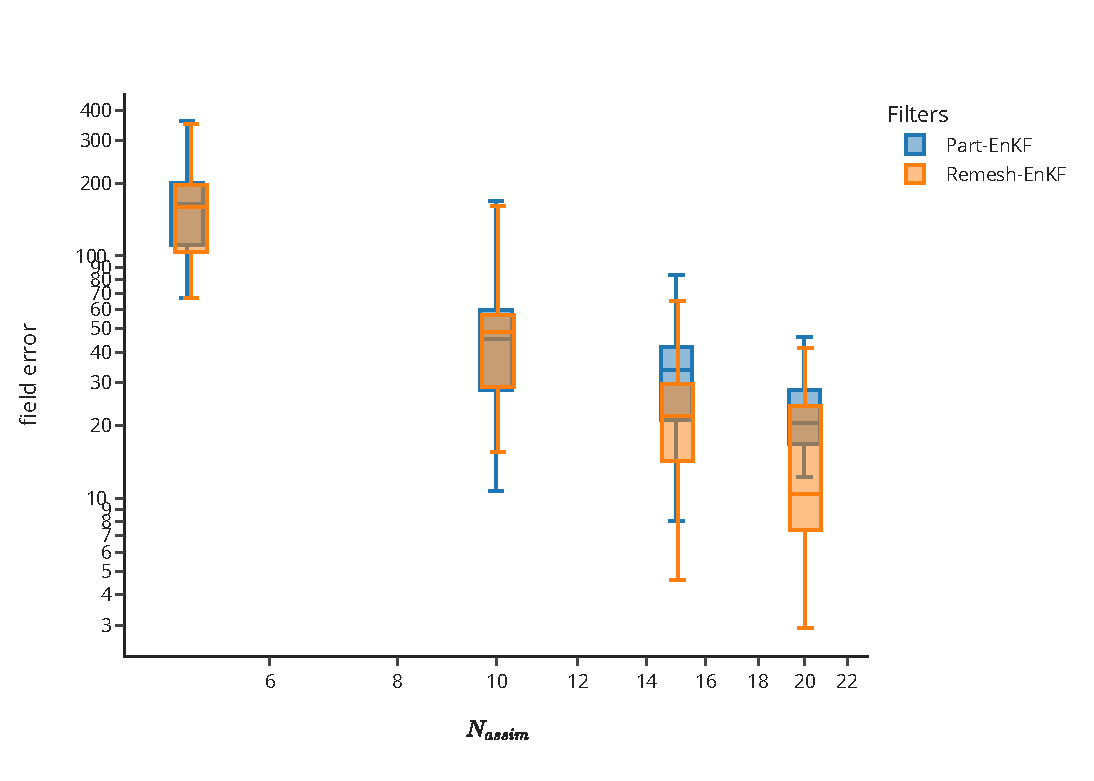
\includegraphics[height=0.40\textheight]{../../conference/images/dipole_results/MSE_na_box_log_log.pdf}
                \end{subfigure}
                \begin{subfigure}{\textwidth}
                    \centering
                    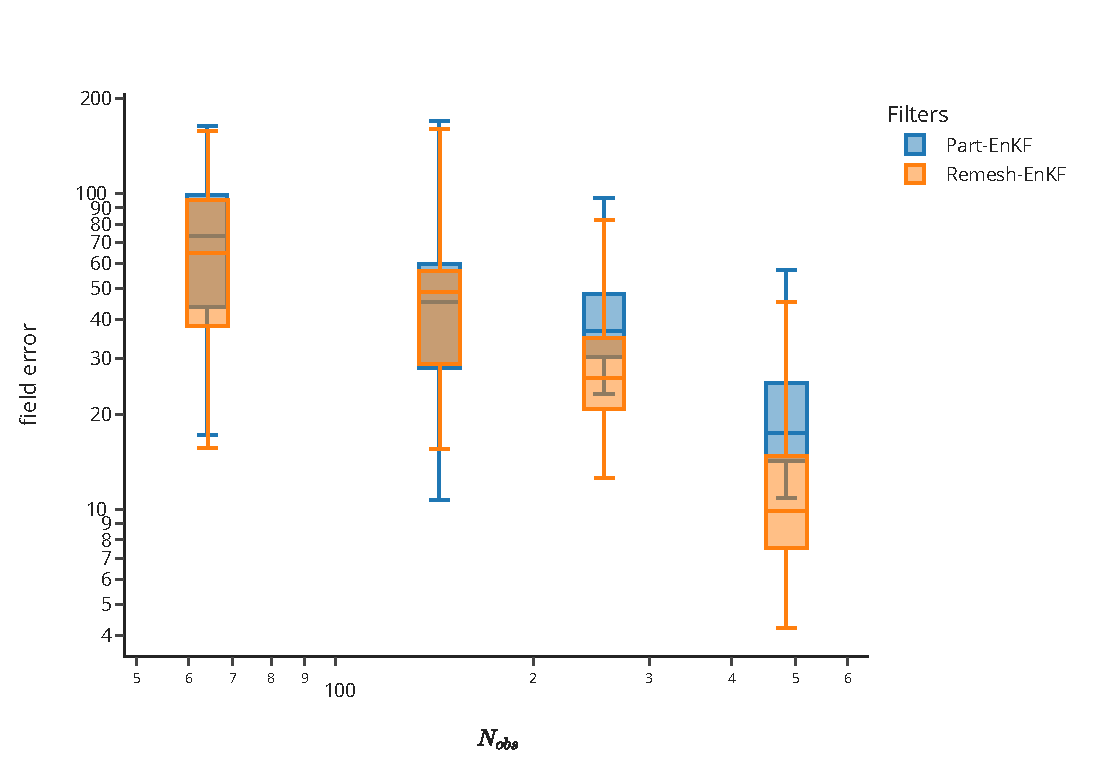
\includegraphics[height=0.40\textheight]{../../conference/images/dipole_results/MSE_nobs_box_log_log.pdf}
                \end{subfigure}
            \end{figure}
        \end{column}
        \begin{column}{0.5\textwidth}
            \begin{figure}
                \begin{subfigure}{\textwidth}
                    \centering
                    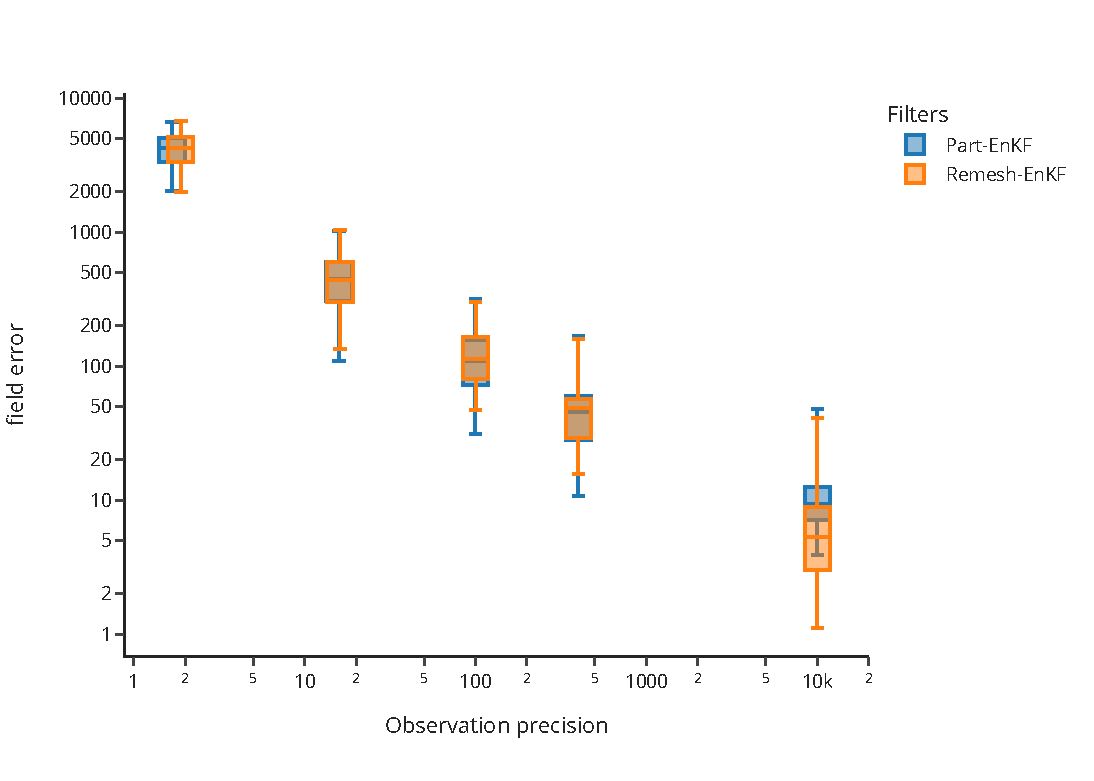
\includegraphics[height=0.40\textheight]{../../conference/images/dipole_results/MSE_obs_precision_box_log.pdf}
                \end{subfigure}
                \begin{subfigure}{\textwidth}
                    \centering
                    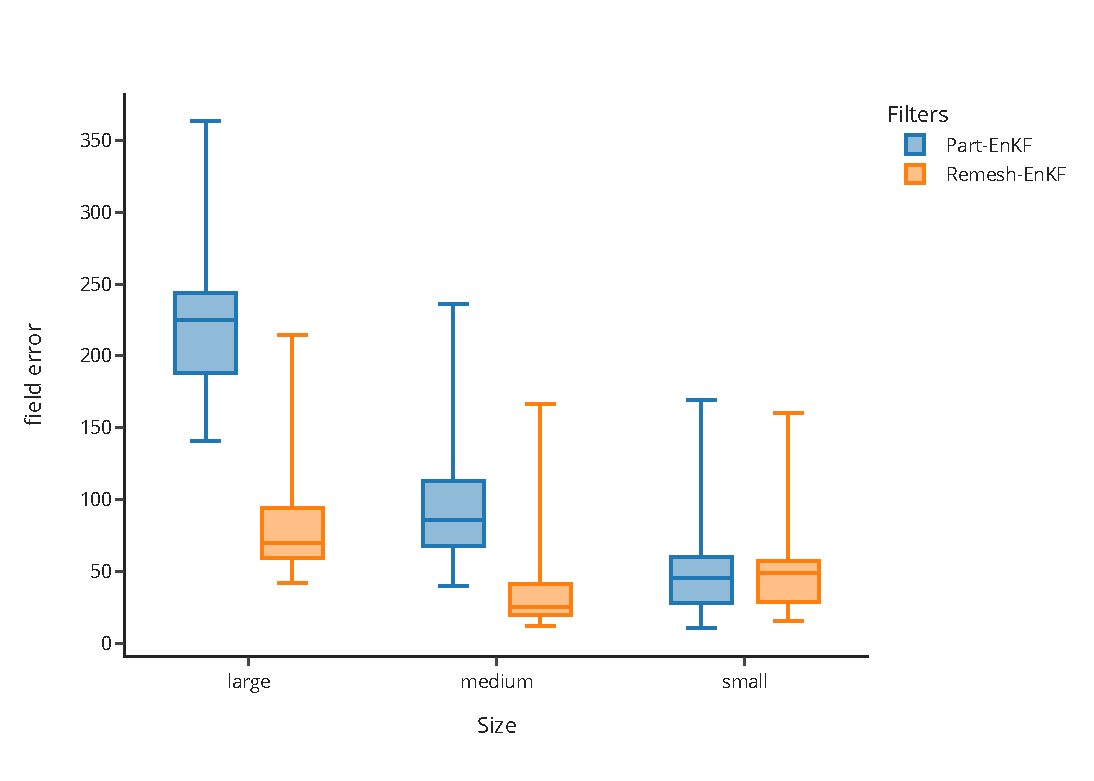
\includegraphics[height=0.40\textheight]{../../conference/images/dipole_results/MSE_size_box.pdf}
                \end{subfigure}
            \end{figure}
        \end{column}
    \end{columns}
\end{frame}


\end{document}